\chapter{Measurement as Minimal Path Collapse}

\section{\texorpdfstring{\textbf{Choosing one worldline from many.}}{13.1 --- Choosing one worldline from many.}}

We have spent the last few chapters building a vocabulary of possibilities. We have explored \textbf{bundles} as clusters of legal futures, \textbf{interference} as the mechanism by which those futures constrain one another, \textbf{curvature} as the shape of the manifold, and \textbf{geodesics} as the optimal paths through rewrite space.

However, a system that only contains *possibilities* is not a computer; it is a daydream. To perform actual computation, the system must eventually commit. We must now address the fundamental question of execution:

\begin{quote}
\textbf{How does a system choose ONE future out of the structured cloud of possibilities?}
\end{quote}

How does Chronos pick a single, razor-thin line through the expanding cone of Kairos? How does the runtime transform the theoretical ``could'' into the historical ``did''?

This phenomenon is called \textbf{collapse}.

It is vital to strip this term of its baggage. This is not quantum collapse. It is not random, spooky, or metaphysical. It does not require a conscious observer or a Schrodinger's cat. In the context of the \COMPUTER{} framework, collapse is a purely geometric operation:

\begin{quote}
\textbf{Selecting the next state by choosing the shortest or most consistent rewrite from an interacting bundle.}
\end{quote}

Let us make that idea precise.

\begin{center}\rule{0.5\linewidth}{0.5pt}\end{center}

\section{\texorpdfstring{\textbf{Collapse is Selection, Not Destruction}}{13.2 --- Collapse is Selection, Not Destruction}}

There is a common misconception that when a decision is made, the unchosen options are destroyed—annihilated from existence as if they never were. In an RMG+DPO universe, this is not the case.

When the runtime collapses a rewrite bundle, it is not performing a probabilistic roll of the dice, nor is it ``measuring'' the state in a quantum sense to force a wavefunction to resolve. Instead, it is exercising a function of \textbf{selection}.

The runtime evaluates the bundle and chooses one legal Double-Pushout (DPO) rewrite that satisfies the system's requirements for consistency, priority, and minimality. The other futures—the roads not taken—do not vanish into non-existence. They remain as \textbf{nearby universes} in Rulial Space. They are valid mathematical objects that simply lie off the axis of the active worldline. They are the shadow paths, the counterfactuals, the branches of the map that exist but remain untraveled by the observer known as Chronos.

In this model, collapse is synonymous with selection, and selection is synonymous with motion. To collapse the wave of possibility is to advance the worldline one tick forward.

\begin{figure}[h]
\centering
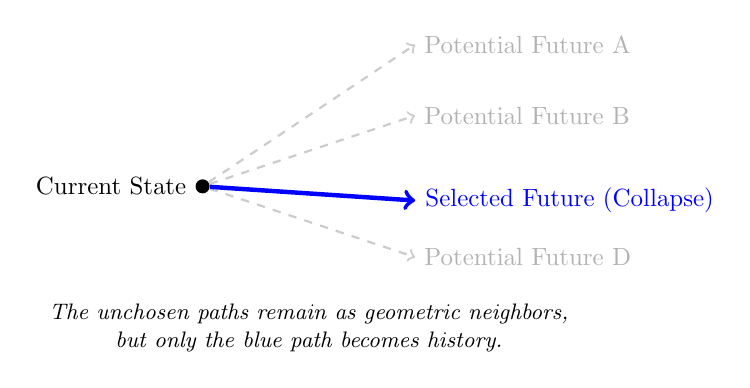
\begin{tikzpicture}[scale=0.9, transform shape]
    % Nodes
    \node[circle, fill=black, inner sep=2pt, label=left:Current State] (Start) at (0,0) {};
    
    % Unchosen paths (faded)
    \draw[->, thick, gray!40, dashed] (Start) -- (3, 2) node[right, gray!60] {Potential Future A};
    \draw[->, thick, gray!40, dashed] (Start) -- (3, 1) node[right, gray!60] {Potential Future B};
    \draw[->, thick, gray!40, dashed] (Start) -- (3, -1) node[right, gray!60] {Potential Future D};
    
    % Chosen path (solid)
    \draw[->, ultra thick, blue] (Start) -- (3, -0.2) node[right, blue] {Selected Future (Collapse)};
    
    % Annotation
    \node[align=center, font=\small] at (1.5, -2) {\textit{The unchosen paths remain as geometric neighbors,}\\ \textit{but only the blue path becomes history.}};
\end{tikzpicture}
\caption{Collapse as Selection: The runtime identifies a bundle of valid rewrites but selects only one to become the active worldline. The others remain as "ghost" neighbors in Rulial Space.}
\end{figure}

\begin{center}\rule{0.5\linewidth}{0.5pt}\end{center}

\section{\texorpdfstring{\textbf{Minimal Path Collapse}}{13.3 --- Minimal Path Collapse}}

If the runtime must choose, how does it decide? It does not flip a coin. It measures distance.

Imagine the bundle of choices as a set of vectors pointing toward different future states. The runtime applies a simple, universal heuristic: \textbf{Choose the rewrite with minimal Rulial Distance relative to the intended path.}

This concept of the ``intended path'' is flexible but rigorous. It might represent the geodesic—the naturally optimal path through the geometry. It might represent a target structure the system is trying to converge upon, or a semantic invariant that must be maintained. It could be defined by type constraints, strict scheduler priorities, or even directives from an external observer.

Regardless of the specific metric, the principle of Minimal Path Collapse ensures that the system favors \textbf{stability}. By consistently choosing the ``cheapest'' or ``closest'' valid move, the system guarantees consistency, determinism, and convergence. It prevents the worldline from jittering chaotically between disparate states.

This is the geometric analog of concepts familiar to computer scientists: greedy evaluation in reduction semantics, shortest-reduction paths in lambda calculus, or optimal lowering in compiler design. It is the canonical ordering of a version control merge. But here, we treat it not as a rule of logic, but as a rule of geometry. The ``closest'' future wins.

\begin{center}\rule{0.5\linewidth}{0.5pt}\end{center}

\section{\texorpdfstring{\textbf{Legal Collapse: The Role of K-Interfaces}}{13.4 --- Legal Collapse: The Role of K-Interfaces}}

We must emphasize that minimality is secondary to \textbf{legality}. A rewrite cannot be chosen simply because it is efficient; it must first be valid.

For a collapse to occur, the rewrite must pass a rigorous gauntlet of structural checks. Its \textbf{L-pattern} must match the current RMG topology perfectly. Its \textbf{K-interface}—the preserved structure—must remain intact throughout the transformation. Its \textbf{R-pattern} must be inserted without tearing the graph, leaving no dangling edges or violated invariants.

Collapse is not merely picking a favorite option; it is picking the cheapest future that does not break the universe. This rigorous filtering is why collapse leads to stability. The system is structurally incapable of picking an illegal universe. It cannot collapse into nonsense because the geometry of the wormholes forbids it.

\begin{center}\rule{0.5\linewidth}{0.5pt}\end{center}

\section{\texorpdfstring{\textbf{Collapse as Constraint Satisfaction}}{13.5 --- Collapse as Constraint Satisfaction}}

We can view the entire process of collapse as a high-speed solver running in the heart of the runtime. At every tick, the system performs a distinct sequence of operations.

First, it identifies the set of all theoretically possible futures. Next, it discards those that are incompatible with the current interface constraints. From the remaining valid set, it applies priorities derived from the structural context or rule definitions. Finally, from this refined list, it selects the single rewrite with the lowest computational cost or Rulial Distance.

This is a \textbf{constraint satisfaction problem} that resolves to a single solution. It is the antithesis of randomness or magic. It is a procedure defined by legality, minimality, and consistency. The runtime is not making arbitrary choices; it is navigating the curvature of the local Rulial Surface, sliding down the gradient of least resistance.

\begin{center}\rule{0.5\linewidth}{0.5pt}\end{center}

\section{\texorpdfstring{\textbf{Collapse and Interference}}{13.6 --- Collapse and Interference}}

In the previous chapter, we observed how bundles interact through interference—how they can conflict with or reinforce one another. Collapse is the moment where that interference crystallizes into reality.

When bundles interfere, the collapse mechanism acts as the final arbiter. Destructive interference effectively removes illegal futures from consideration before the selection process even begins. Constructive interference, on the other hand, highlights the stable options, effectively deepening the "grooves" in the manifold that guide the selection.

This dynamic explains why well-designed systems appear to "naturally converge" on correct solutions: their rules are designed to interfere constructively, making the correct path the path of least resistance. Conversely, fragile systems explode because their rules interfere destructively, leaving the collapse mechanism with no good options—or only options that lead to high-entropy states. Collapse simply makes the invisible geometry of interference visible.

\begin{center}\rule{0.5\linewidth}{0.5pt}\end{center}

\section{\texorpdfstring{\textbf{Collapse is the Deterministic Arrow of Computation}}{13.7 --- Collapse is the Deterministic Arrow of Computation}}

Collapse provides computation with its directionality. Before the moment of collapse, the system exists in a state of potentiality: many possible futures, many adjacent universes, and many overlapping bundles of rewrites.

After collapse, there is singularity: exactly one next world, exactly one tick of the clock, exactly one continuation.

This transition defines the \textbf{Arrow of Computation}:
\[ \text{BUNDLE} \rightarrow \text{COLLAPSE} \rightarrow \text{WORLDLINE ADVANCE} \]

This arrow is the fundamental mechanism behind everything we recognize as execution. It is the engine of control flow, scheduling, evaluation order, and compiler lowering. Without collapse, a system is merely a static map of possibilities. With collapse, it becomes a traveler moving through the territory. Collapse is the beating heart of computation.

\begin{figure}[h]
\centering
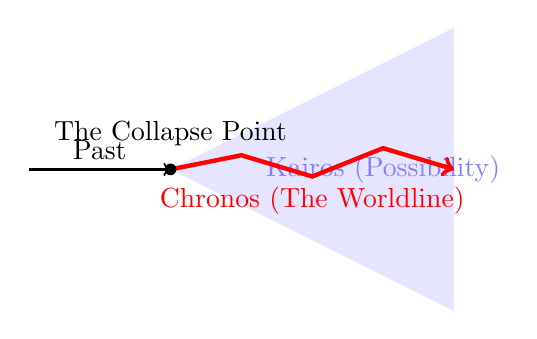
\begin{tikzpicture}[scale=0.9]
    % Cone of Possibility
    \fill[blue!10] (0,0) -- (4,2) -- (4,-2) -- cycle;
    \node[blue!50] at (3,0) {Kairos (Possibility)};
    
    % The Path
    \draw[thick, ->] (-2,0) -- (0,0);
    \draw[ultra thick, red, ->] (0,0) -- (1, 0.2) -- (2, -0.1) -- (3, 0.3) -- (4, 0);
    
    % Labels
    \node[above] at (-1,0) {Past};
    \node[below, red] at (2, -0.1) {Chronos (The Worldline)};
    \node[circle, fill=black, inner sep=1.5pt] at (0,0) {};
    \node[above] at (0,0.2) {The Collapse Point};

\end{tikzpicture}
\caption{The Arrow of Computation: The system constantly moves from the singular Past, through the Collapse Point, picking one specific path through the widening cone of Possibility (Kairos) to create the Worldline (Chronos).}
\end{figure}

\begin{center}\rule{0.5\linewidth}{0.5pt}\end{center}

\section{\texorpdfstring{\textbf{Collapse as Structured Information Loss}}{13.8 --- Collapse as Structured Information Loss}}

It is important to acknowledge that collapse is inherently a process of loss. In selecting one path, the system discards most futures, most rewrites, and most local possibilities.

However, we must distinguish this from entropy. This is not the disorderly loss of information associated with heat death or noise. This is \textbf{structured pruning}. It is the deliberate act of choosing one path out of a structured set and discarding the others precisely because they violate the requirements of consistency or minimality.

The information lost consists only of the ``forks'' you didn't take. As we established, they remain as neighbors in Rulial Space, accessible in theory but abandoned in the specific history of the current execution.

\begin{center}\rule{0.5\linewidth}{0.5pt}\end{center}

\section{\texorpdfstring{\textbf{Collapse \& Optimal Computation}}{13.9 --- Collapse \& Optimal Computation}}

Finally, we see that collapse is the mechanism by which optimization emerges. It is not just about being deterministic; it is about being optimal.

Because the collapse mechanism is biased toward the minimal, legal, and consistent path, systems naturally tend toward canonical forms. Normalization stabilizes and evaluation converges not because of external heuristics, but because the geometry of the collapse favors these states. It is the process by which a system ``falls'' into its correct answer.

\begin{center}\rule{0.5\linewidth}{0.5pt}\end{center}

\section*{\textbf{FOR THE NERDS\texttrademark}}

\section{\texorpdfstring{\textbf{Collapse, Confluence, and Canonical Forms}}{13.10 --- Collapse, Confluence, and Canonical Forms}}

For those versed in formal rewrite theory, the concept of collapse is deeply intertwined with established mathematical properties. It relates intimately to \textbf{confluence} (the Church-Rosser property), critical pair resolution, and normalization (both weak and strong). It mirrors concepts of orthogonality, peak reduction, and standardization theorems.

However, \COMPUTER{} extends these abstract concepts into the realm of geometry. In our framework, ``peak sets'' become bundles. ``Critical pairs'' are understood as interference patterns. ``Standardization'' is simply the selection of the minimal path. The ``reduction sequence'' is the worldline itself. By mapping confluence onto a metric space, we sharpen the abstract algebra of rewriting with the precise tools of geometry.

\textit{(End sidebar.)}

\begin{center}\rule{0.5\linewidth}{0.5pt}\end{center}

\section{\texorpdfstring{\textbf{Transition: From Collapse to the Arrow of Computation}}{13.11 --- Transition: From Collapse to the Arrow of Computation}}

We have now explained the mechanics of bundles, interference, and collapse. We understand how the system chooses a step. But this raises a profound question regarding the arrow of time itself.

Why does collapse \emph{always} move forward? Why is it that we cannot simply un-collapse, rewind time, or undo computation with the same ease that we perform it?

It turns out that \textbf{reversibility and irreversibility are structural, emergent properties of the RMG universe.}

And that is the subject of \textbf{Chapter 14}.
